\documentclass{article}
 
\usepackage{color}
\usepackage{listings}
\usepackage{graphicx}
\usepackage{subfig}

\definecolor{MyYellow}{rgb}{1,1,0.8}
 
\lstset{language=Matlab,backgroundcolor=\color{MyYellow},basicstyle=\footnotesize,numberstyle=\footnotesize,numbers=left,stepnumber=1,numbersep=5pt,breaklines=true,frame=lines,tabsize=2}
 
\author{Ruurd Moelker \and Jan Paul Posma}
\date{\today}
\title{Signalen \& Systemen \\Practicum 2}

\begin{document}
\maketitle
 
\section{Opgave 1}
In dit practicum worden geluiden geproduceerd met behulp van frequentiemodulatie volgens de functie:
$$x(t) = A(t)cos(2 \pi f_c t + I(t)cos(2 \pi f_m t + \phi_m) + \phi_c)$$
$A(t)$ en $I(t)$ worden gegeven door middel van:
$$A(t) = A_0~exp(\frac{-t}{\tau})$$
$$I(t) = I_0~exp(\frac{-t}{\tau})$$
De functies zijn gelijk op de factoren $A_0$ en $I_O$ na. De  exponenti\"ele afname van van beide functies worden berekend met behulp van de functie bellenv, verantwoordelijk voor het gedeelte $exp(\frac{-t}{\tau})$ bij het berekenen van $A(t)$ en $I(t)$. De functie bellenv wordt hieronder gegeven.

\begin{lstlisting}
function [tt, yy] = bellenv(tau, dur, fsamp);
%BELLENV produces envelope function for bell sounds
%
% usage: [tt,yy] = bellenv(tau, dur, fsamp);
%
% input:
%            tau = time constant
%            dur = duration of the envelope
%          fsamp = sampling frequency
% output:
%             tt = time axis
%             yy = decaying exponential envelope
%
%   note: produces exponential decay for positive tau

tt = 0:1/fsamp:dur;
yy = exp(-tt/tau);

end
\end{lstlisting}

\section{Opgave 2}
Hieronder staat de functie playfm. 

\begin{lstlisting}
function xx = playfm( fc, fm, fic, fim, A0, I0, tau, dur, fsamp )
%function calculates fm  function with given values. After which the created sound is played.

[tt, yy] = bellenv(tau, dur, fsamp);
At = A0 * yy;
It = I0 * yy;

xx = At .* cos((2*pi*fc*tt) + fic + (It .* cos(2*pi*fm*tt + fim)));
soundsc(xx, fsamp);

end
\end{lstlisting}

De gebruikte invoer bij deze functie is als volgt: $f_c = 110$, $f_m = 220$, $\phi_c = 0$, $\phi_m = 0$, $A_0 = 10$, $I_0 = 10$, $\tau = 2$, $T_{dur} = 6$, $F_s = 11025$. Playfm levert een bell geluid op als de frequentie van carrier en messenger zich verhouden als 1:2. Een verhoging danwel verlaging van de waarde $I_0$ heeft respectievelijk een scherper danwel doffer geluid ten gevolge. Dit komt omdat bij een hoge $I_0$ waarde de hoge tonen minder snel dempen dan bij een lage $I_0$ waarde.

\section{Opgave 3}
Opdracht 3 hebben wij uitgevoerd voor case 1 en case 5. Om duidelijke spectogrammen te maken hebben we de functie spectro gemaakt. De functie spectro is als volgt:

\begin{lstlisting}
function spectro( xx )
%function creates clear spectogram for an input with a sampling rate of 11025

[S,F,T] = spectrogram(xx, 1102, 1000, 1024, 11025);
imagesc(T, F, abs(S))
axis xy

end
\end{lstlisting}

\subsection{case 1}
a)\\
De combinatie van $f_c = 220$ en $f_m = 440$ heeft tot gevolg een signaal met de frequentie $f_s$, gegeven door $f_s = 440 \pm 220 = {220, 660}$. $f_s$ bevat ook veelvouden van de eerder gevonden waarden. De fundamentele frequentie is de ggd van alle frequenties in het signaal, dus $ggd(220, 660) = 220$. Verificatie van de fundamentele frequentie kan gebeuren door alle frequenties in het signaal te delen door de fundamentele frequentie, waarbij de uitkomst altijd een geheel getal moet zijn.

b)\\
Een hogere $I_0$ zorgt ervoor dat frequentie minder snel dempen. Hierdoor klinkt het geluid scherper. Bij een lage $I_0$ zijn dezelfde frequenties actief als bij een hoge $I_0$, maar deze sterven zo snel uit dat het geluid dof klinkt. Dit is grafisch nog eens te zien in figuur \ref{fig:case1b}.

\begin{figure}[h]
  \centering
  \subfloat[][$I_0 = 1$]{\label{fig:b1i1}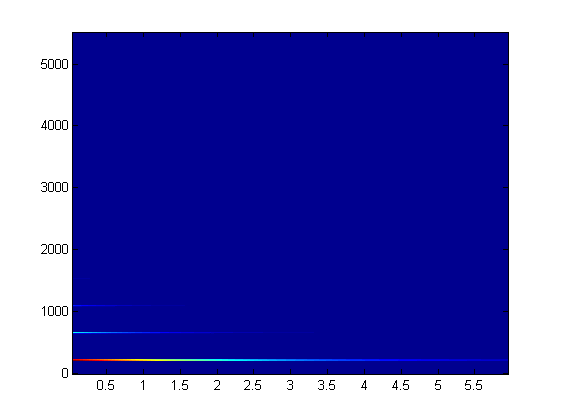
\includegraphics[width=0.4\textwidth]{content/b1i1.png}}                
  \subfloat[][$I_0 = 5$]{\label{fig:b1i5}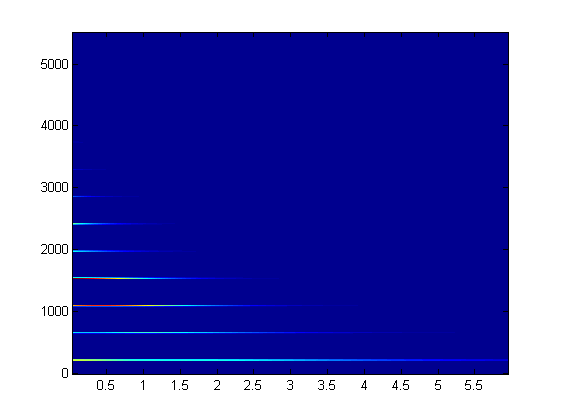
\includegraphics[width=0.4\textwidth]{content/b1i5.png}}
  \subfloat[][$I_0 = 10$]{\label{fig:b1i10}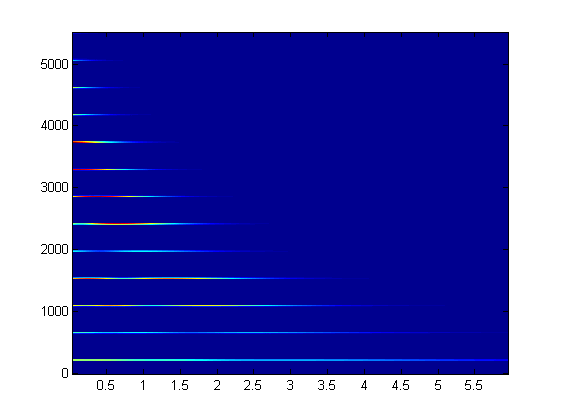
\includegraphics[width=0.4\textwidth]{content/b1i10.png}}
  \caption{Geval 1 met verschillende $I_0$ waardes}
  \label{fig:case1b}
\end{figure}


c,d)\\
Het signaal begint te alterneren tussen $A_0$ en $-A_0$, dus 1 en -1, en na 6 seconden zou deze moeten alterneren tussen 0.0498 en -0.0498 (namelijk $e^\frac{-t}{\tau} = e^\frac{-6}{2}$).\\
\\
De variatie in de frequentie neemt af in de tijd, ten gevolge van het afnemende karakter van $I(t)$. Daardoor lijkt het steeds meer op een gewone cosinus.
\begin{figure}[h]
  \centering
  \subfloat[][opdracht c]{\label{fig:c1}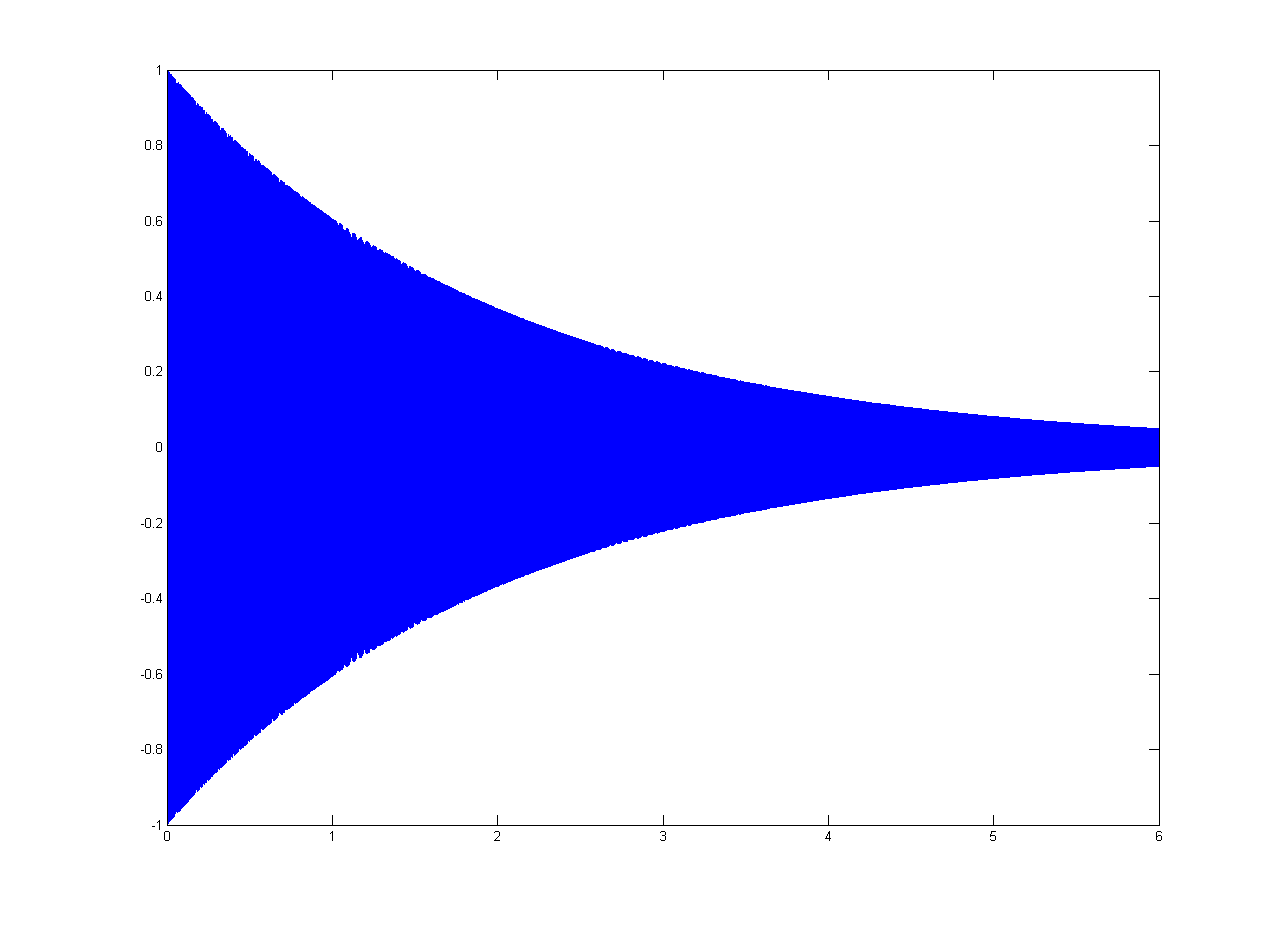
\includegraphics[width=0.5\textwidth]{content/c1.png}}
  \subfloat[][opdracht d]{\label{fig:d1}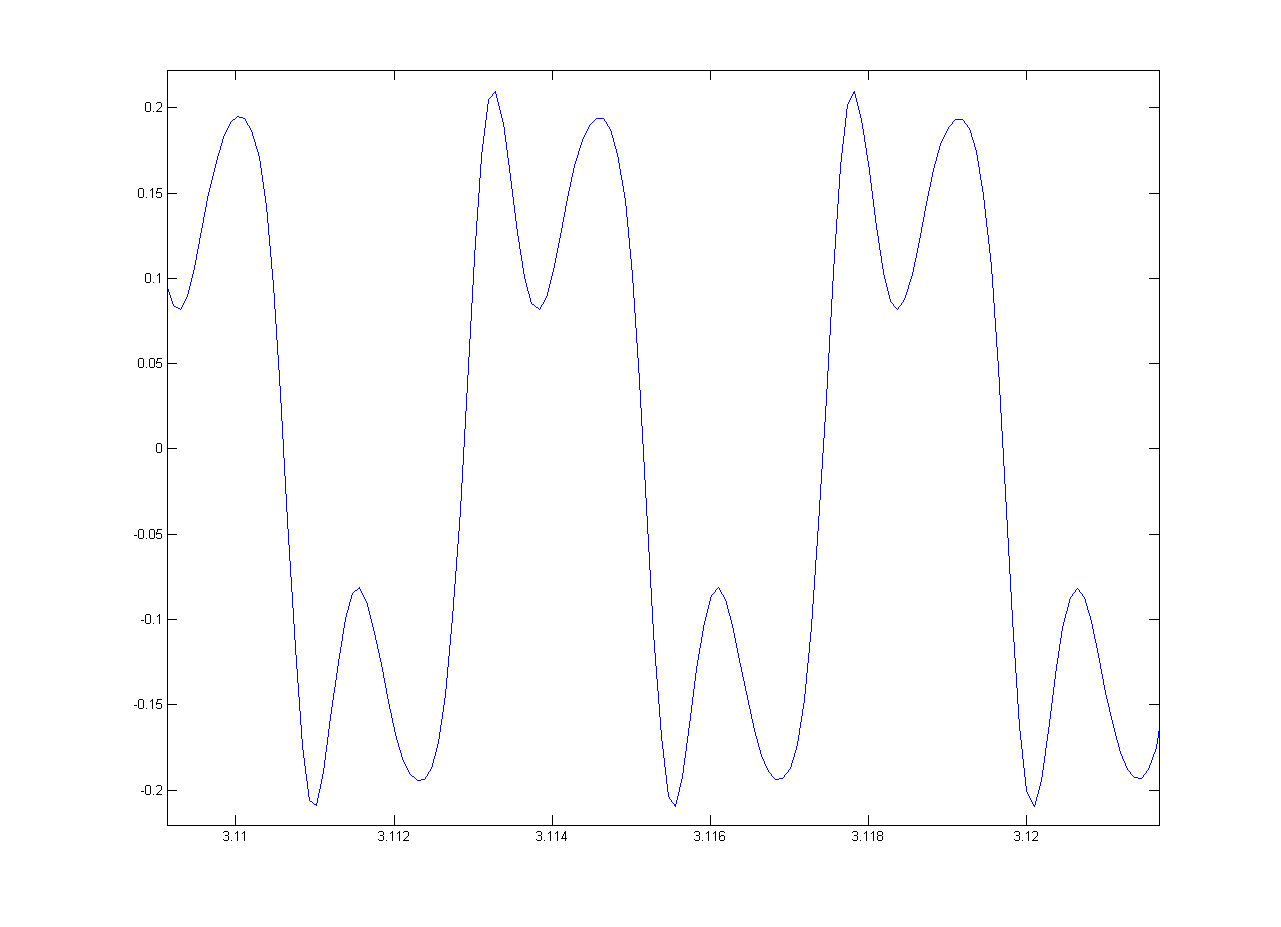
\includegraphics[width=0.5\textwidth]{content/d1.png}}
  \caption{Opdracht c en d voor geval 1}
  \label{fig:case1b}
\end{figure}

\newpage 
\subsection{case 5}
a)\\
De combinatie van $f_c = 250$ en $f_m = 350$ heeft tot gevolg een signaal met de frequentie $f_s$, gegeven door $f_s = 350 \pm 250 = {100, 600}$. $f_s$ bevat ook veelvouden van de eerder gevonden waarden. De fundamentele frequentie is de ggd van alle frequenties in het signaal, dus $ggd(100, 600) = 100$. Ook hier kan de fundamentele frequentie geverificeerd worden door door alle frequenties in het signaal te delen door de fundamentele frequentie, waarbij de uitkomst altijd een geheel getal moet zijn.

b)\\
De waarde van $I_0$ heeft een gelijke invloed als bij de eerste case. Een hoge $I_0$ geeft een scherp geluid, een lage $I_0$ een dof geluid. In figuur \ref{fig:case5b} staat de invloed van $I_0$ op spectogrammen afgebeeld.

\begin{figure}[h]
  \centering
  \subfloat[][$I_0 = 1$]{\label{fig:b5i1}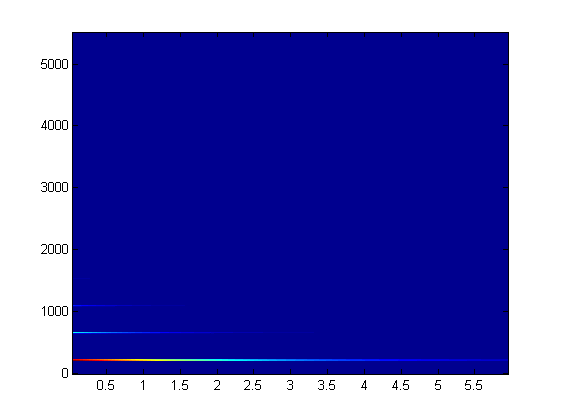
\includegraphics[width=0.4\textwidth]{content/b5i1.png}}                
  \subfloat[][$I_0 = 3$]{\label{fig:b5i3}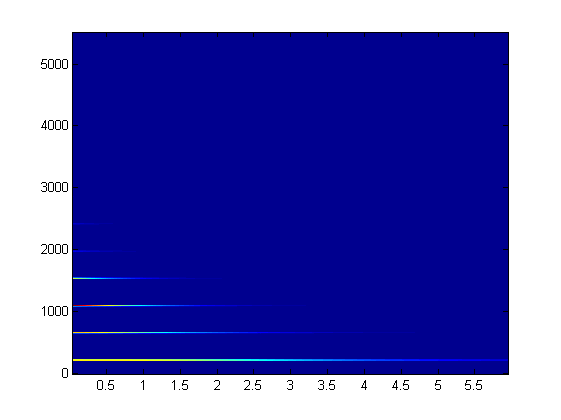
\includegraphics[width=0.4\textwidth]{content/b5i3.png}}
  \subfloat[][$I_0 = 10$]{\label{fig:b5i10}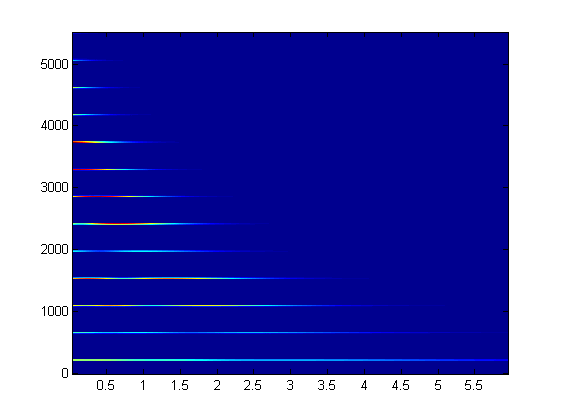
\includegraphics[width=0.4\textwidth]{content/b5i10.png}}
  \caption{Geval 5 met verschillende $I_0$ waardes}
  \label{fig:case5b}
\end{figure}

c,d)\\
Het signaal begint te alterneren tussen $A_0$ en $-A_0$, dus 1 en -1, en na 5 seconden zou deze moeten alterneren tussen 0.00674 en -0.00674 (namelijk $e^\frac{-t}{\tau} = e^\frac{-5}{1}$).\\
\\
De variatie in de frequentie neemt wederom af in de tijd, waardoor het steeds meer op een cosinus lijkt.
\begin{figure}[h]
  \centering
  \subfloat[][opdracht c]{\label{fig:c5}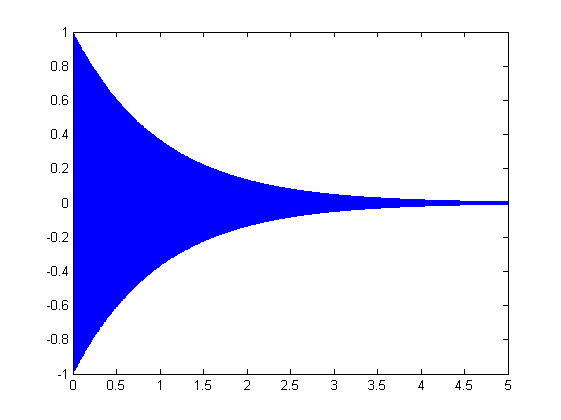
\includegraphics[width=0.5\textwidth]{content/c5.png}}
  \subfloat[][opdracht d]{\label{fig:d5}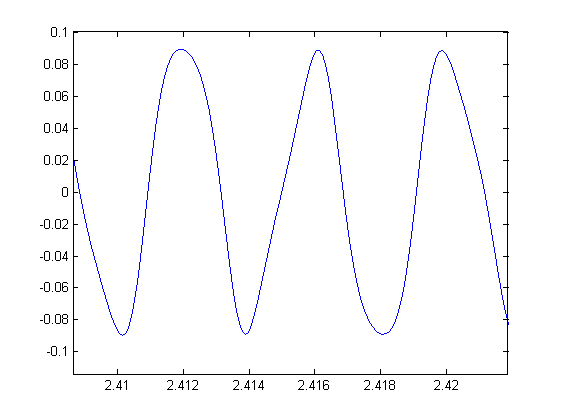
\includegraphics[width=0.5\textwidth]{content/d5.png}}
  \caption{Opdracht c en d voor geval 5}
  \label{fig:case1b}
\end{figure}


\end{document}